\documentclass{article}
\usepackage{graphicx}
\usepackage{amsmath}
\usepackage{xcolor}
\begin{document}

\title{\textbf{READ ME:} A Map of the Local Velocity Substructure in the Milky Way Disk}
\author{\textit{Alan Pearl}\\
  \texttt{alanpearl13@gmail.com}}
 \date{\today}
\maketitle

\section{Overview}

This paper contains a detailed explanation of the procedure used in the paper \textit{A Map of the Local Velocity Substructure in the Milky Way Disk} (\texttt{Paper/ms.pdf}). During this project, I created the most accurate proper motion correction algorithm to date, which can remove systematic error at very small scales, and estimate how much error is remaining. I used this to calculate three dimensional velocities of Disk stars and find substructure in the motion of the Disk. I will explain the required format of the observational data files, and how to use them with my codes to recreate all of the results and figures. 

My codes are entirely written in Python, and scripted with Bash. In order for my codes to work, you must be able to execute Python~2.7.12 from \texttt{/usr/bin/python2} and Bash from \texttt{/bin/bash}. Make sure the Python modules NumPy, PyFITS, and matplotlib are installed. I recommend using a Unix system, but it is probably possible to run this on Windows using Cygwin or something similar.

At the beginning (alphabetically) of each directory, there may be one or several Bash scripts whose names begin with a number and end with \texttt{.sh}. These scripts call Python codes and contain comments explaining what they do. During each section of this paper, I will reference a relevant shell script, and I recommend following along with it while I describe the codes that it calls.

Before running any of my codes, you must first make a new folder called \texttt{data} (i.e. \fcolorbox{lightgray}{lightgray}{\texttt{mkdir data}}). Then, download the file \texttt{datafiles.tar.gz}\footnote{\texttt{https://drive.google.com/open?id=0B83JqdngCoUBVDk4a2t2dVE3OGM}}, and place it in the newly created \texttt{data/} directory. Then, to run the entire procedure and make all figures, all you need to do is execute the shell (Bash) script located in the top directory, \texttt{1main.sh} (you can do this with the command \fcolorbox{lightgray}{lightgray}{\texttt{source 1main.sh}} or \fcolorbox{lightgray}{lightgray}{\texttt{./1main.sh}}). This script uncompresses the data files, gives permission for all of my codes to be executed, and then runs them all (the three main scripts that it calls are explained in the next three sections). My code may raise some warnings about invalid values, but it should all work -- otherwise, there is some serious compatibility issue. Note that some of the codes which require searching for nearby objects have very long execution times (\texttt{qso/nearestpmfit.py}, \texttt{qso/mk\_pearl\_corr.py}, and \texttt{qso/dist\_vs\_match.py}).

In the scripts, when I call my codes, I use lots of arguments, which generally follow the same usage. Each argument, separated by a space, can set the value of the variable within the code of the same name to the given string (e.g.\ the argument \texttt{infile=coords.fits} sets the variable \texttt{infile} to the string \texttt{"coords.fits"}). Additionally, I can set a boolean variable to \texttt{True} with an argument starting with a dash (e.g.\ the argument \texttt{-overwrite} sets the variable \texttt{overwrite} to \texttt{True} -- I usually use this particular argument to stop my code from prompting me to come up with a new filename during a file conflict). In the actual code, the arguments are usually read through the function \texttt{read\_argv(sys.argv)} and updated to the variables with the function \texttt{vars().update(...)}. This helps cut down on the number of Python codes I need to write when I only want a slight change. To remove additional clutter in directories containing Python codes, I keep the data files in the \texttt{data/} directory, but this is just my preference.

\section{Proper Motion Correction (\texttt{qso/})} \label{sec:qso}

The \texttt{qso/} directory works with the extragalactic data (note that extragalactic objects are very far away, and therefore their proper motion measurements should be only due to random and systematic error -- our goal is to remove the systematic error). It contains all the code needed to create the proper motion correction table, as well as all relevant figures. The procedure explained in this section generally follows what is done in the script \texttt{1qso.sh} (the codes called in this script will take about an hour to run).

Jeff Carlin sent me a .csv file of QSO's \texttt{dr3dr4q1q2\_qso....csv} and another of galaxies \texttt{dr3dr4q1q2\_galaxy....csv} (they should now be in the \texttt{data/} directory) from LAMOST, which I combine using \texttt{combine\_gal\_qso.py}. This returns a file called \texttt{qagcoords.fits} (quasars and galaxies). This file satisfies the following requirements: it is a .fits file containing extragalactic objects is required, with the headers \texttt{"ra"} (right ascension in degrees), \texttt{"dec"} (declination in degrees), \texttt{"pmra"} (proper motion in right ascension in mas/yr), and \texttt{"pmde"} (proper motion in declination in mas/yr).

The code \texttt{nearestpmfit.py} is essentially a test for the code which makes the actual correction table. It takes in a data file of extragalactic data (such as \texttt{qagcoords.fits}), cuts the data at a specified magnitude of proper motion (via the \texttt{pmcut} argument), deletes duplicates, and corrects the proper motion for each object by subtracting the average proper motion of its nearest neighbors. A new file is returned, which is the same as the old one, but with corrected proper motions \texttt{"pmra\_pearl"} and \texttt{"pmde\_pearl"}, as well as the remaining systematic error estimates \texttt{"pmra\_se"} and \texttt{"pmde\_se"}. I actually run this code twice -- the first time only to get rid of the duplicates and remove quasars with greater absolute proper motion than 30 mas/yr, and the second time to actually test my algorithm on the data. The second time, I write the file \texttt{qagcoords\_ltpm30.fits}, which is used to create several figures.

The code \texttt{mk\_pearl\_corr.py} creates the actual correction table. It determines the correction values at the center of each bin in a grid across right ascension and declination, and returns them as a .fits file. The range of the table spans in right ascension and declination are given via the arguments \texttt{ralim} and \texttt{declim}, respectively. The number of bins in each component are given with the argument \texttt{shape}.

Using the output of \texttt{mk\_pearl\_corr.py}, which I call \texttt{pearl\_corr.fits}, the correction can be quickly implemented to many objects. This will be done in the next section, via the code \texttt{add\_pearl\_corr.py}. \texttt{pearl\_corr.fits} is also presented directly in the paper in Table~2 and Figure~7.

Finally, in order to make Figure 5 (which demonstrates the correlation in proper motion between objects close together in the sky), a large data file called \texttt{dist\_vs\_match.fits} is required. To create the data file, I use the code \texttt{dist\_vs\_match.py}. There are some tricky arguments for this code that I use to randomly cut out some of the data and run a bit quicker: \texttt{datapercent} and \texttt{search0}. \texttt{datapercent} determines the percentage of objects we look for neighbors around (greater than 50 is not really necessary, because most of the extra data at that point will be duplicates, since each neighbor of an object will also find that object as its neighbor). For each object we select, each neighbor within \texttt{search0} degrees is guaranteed to be found (and none will be found further than \texttt{searchmax=5} degrees away). The search radius is then randomly chosen such that approximately the same number of neighbors will be found at all radii above \texttt{search0}. Much more neighbors are likely to be found, even at greater radii, if \texttt{search0} is increased.

\section{Stellar Data (\texttt{stars/})}

The \texttt{stars/} directory works with the stellar data which I use to measure the velocity substructure of the disk. The procedure explained in this section generally follows what is done in the script \texttt{1stars.sh}.

The data file \texttt{dr3\_dr4q1q2\_stellar....fits} contains stellar data from LAMOST, in addition to positionally matched proper motions from PPMXL, and distance calculations based on the K- and r-band absolute magnitude estimates from Jeff Carlin. He sent me this file last summer, so he probably has even more data now if you ask him. His catalog conveniently comes with a readme pdf which explains each column. The RAVE stellar data file \texttt{RAVE\_DR5.fits} was not used in my paper, but I do make some use of it in Section~\ref{sec:futurework}.

In order to make the LAMOST data compatible with my code that transforms its coordinates, it must use all of the correct header names. In the code \texttt{mkLAMOST.py}, I boil down the data into what is necessary, slightly change a few header names, and find the error weighted mean of Carlin's two distance calculations. This returns the file \texttt{LAMOST.fits}, which now just needs my proper motion correction to be implemented.

The code \texttt{add\_pearl\_corr.py} uses my proper motion correction table (created in Section~\ref{sec:qso} -- \texttt{pearl\_corr.fits}) to calculate corrected values for each star in a file. The file must be a .fits file which contains proper motion columns for each component, with headers \texttt{"pmra"} and \texttt{"pmde"} and a position given by columns with headers \texttt{"ra"} and \texttt{"dec"}. I use this code to add correction values to \texttt{LAMOST.fits}.

The code \texttt{mkcoords.fits} contains some useful functions which transform the data from observational coordinates and velocities to Galactocentric Cylindric coordinates, which is what I use in my paper. In the script \texttt{1stars.sh}, I call this code with the \texttt{-Fonly} argument (this removes any star not designated as an F star, which preserves direct comparability with Carlin et al. 2013). The flag \texttt{-elimsys} allows the removal of stars due to systematic error (by default, this removes anything with: $V_R > 8$~km~s$^{-1}$ or $V_\theta > 10$~km~s$^{-1}$ or $V_Z > 10$~km~s$^{-1}$). The flag \texttt{-pearl\_corr\_only} only uses proper motions corrected by my correction, instead of using the Vickers corrections where there is no Pearl correction, or where it contains a large uncertainty.

The code \texttt{spatialbins.py} bins all of the stellar data into three-dimensional bins in $R$, $\theta$, and $Z$, approximately $0.2$~kpc wide on each side. This is used directly in Figure~11. Figure~12 also uses this data, but it averages over one axis at a time via the code \texttt{metabins.py}.

\section{Making the Figures (\texttt{Paper/})}

The \texttt{Paper/} directory contains my paper \textit{A Map of the Local Velocity Substructure in the Milky Way Disk}. In order to make the figures used in this paper, simply run the script \texttt{1figures.sh}. This script requires that the entire procedure from the last two sections is complete, and the necessary data files have been made. This script calls codes which are used to create the figures, which should be looked through individually if you wish to make similar plots.

Each figure is made using matplotlib, some of which use fairly complicated methods. A very good understanding of the matplotlib is important if you wish to alter these figures, especially since many of the figure making codes are pretty messy. If there is any major confusion, send me an email and I will probably be able to help.

\section{Comparison of Different Stellar Data Sets} \label{sec:futurework}

The work I have done since submitting the paper has been adding more data to what we currently have. In the paper, I only selected F stars from LAMOST, but since the distance calculations we are using is now independent of star type, we can extend this to all of the LAMOST stellar data.

Additionally, I downloaded the RAVE Data Release 5 file in the \texttt{stars/} directory. Since RAVE observes in lower declination regions of the sky than LAMOST does, with only a small overlap region, this data gives us data in regions where we had none before. It fills in some of the gap in the southern second quadrant, and third quadrant. Combining this with the LAMOST data might therefore allow us to make justifiable claims about the motion of the disk at lower Galactocentric radii than the Sun ($R<8$~kpc).

In the \texttt{qso/} directory, I included two scripts which overwrite some of the star data files and recreates the velocity substructure figures using different sets of data. \texttt{2LAMOST.sh} (Figures~\ref{fig:sideviewL}~and~\ref{fig:stepthetaL}) does this using all of the LAMOST data, as opposed to only the F stars. \texttt{3RAVE.sh} does this using only RAVE data (Figures~\ref{fig:sideviewR}~and~\ref{fig:stepthetaR}). Note that I shift the allowed Galactocentric radius selection and axis range for the RAVE data to include all of it. If you do this for the LAMOST data as well, you will get an additional sparse region of data with $R < 8$~kpc.

Combining both data sets is very simple after you have called the code \texttt{combine\_LAMOST-RAVE.py}. When calling the code \texttt{mkcoords.py}, just don't use any of the arguments that select a particular set of data (\texttt{-Fonly}, \texttt{-LAMOSTonly}, or \texttt{-RAVEonly}), and it should all be included automatically in the coordinate file \texttt{coords.fits}. The more difficult task would then be figuring out a better way to display the larger region of data. You will need to either make changes to the figure making codes (experimenting with different values for the \texttt{figsize} keyword during the matplotlib figure creation will probably be necessary) or think of different ways to present the data and make new scripts for that.

I currently do not have any Pearl correction values outside of the region covered by LAMOST, since this is where I get my extragalactic data from. Therefore, I make no attempt of correcting for RAVE data, since there is little overlap, and instead use the Vickers-corrected values. I have a function inside \texttt{combine\_LAMOST-RAVE.py} to calculate the Vickers-corrected values.

Finally, we will probably want to eventually add even more datasets to what we are currently using, like Gaia (at some point, the amount of data may become too large, and we may need to randomly select stars to remove from regions where there is more than enough). Whenever you add new stellar data, you will probably need to write a script similar to \texttt{combine\_LAMOST-RAVE.py} to combine it with the rest of the data. Making sure all of the header strings and units are correct is essential if you wish to transform the coordinates correctly with the code \texttt{mkcoords.py}. Note that I use units of kpc for distance (RAVE had to be converted from pc) and mas/yr for proper motion, where $\texttt{pmra} = \mu_\alpha \cos{\delta}$ and $\texttt{pmde} = \mu_\delta$.

\begin{figure}
\centering
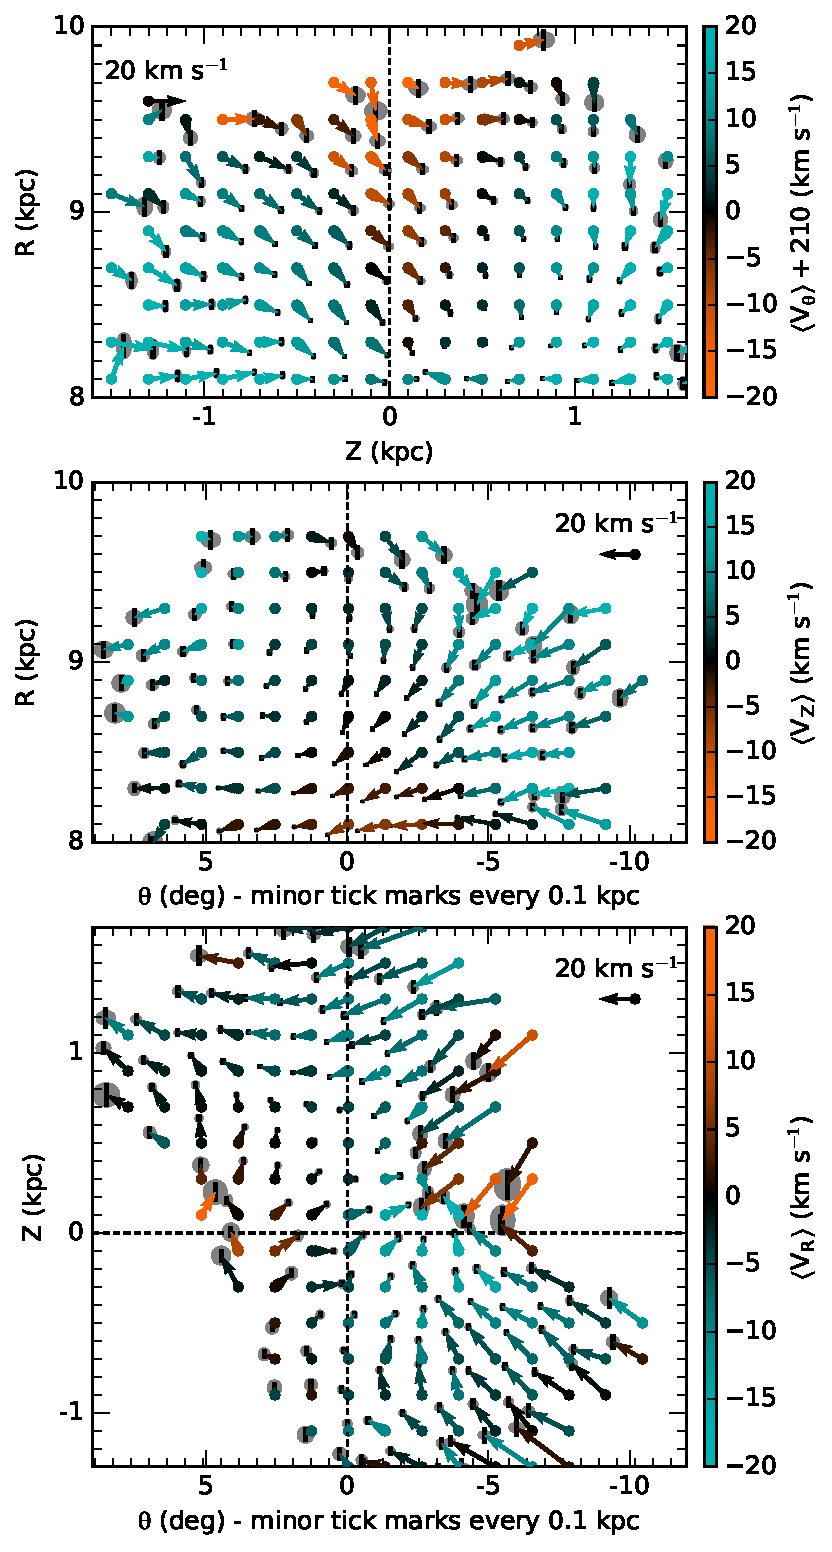
\includegraphics[width=.7\textwidth]{sideviewL.pdf}
\caption{
	Comparable to Figure~10 in my paper, but contains all LAMOST stellar data, instead of only F stars. 
	\label{fig:sideviewL}
}
\end{figure}

\begin{figure}
\centering
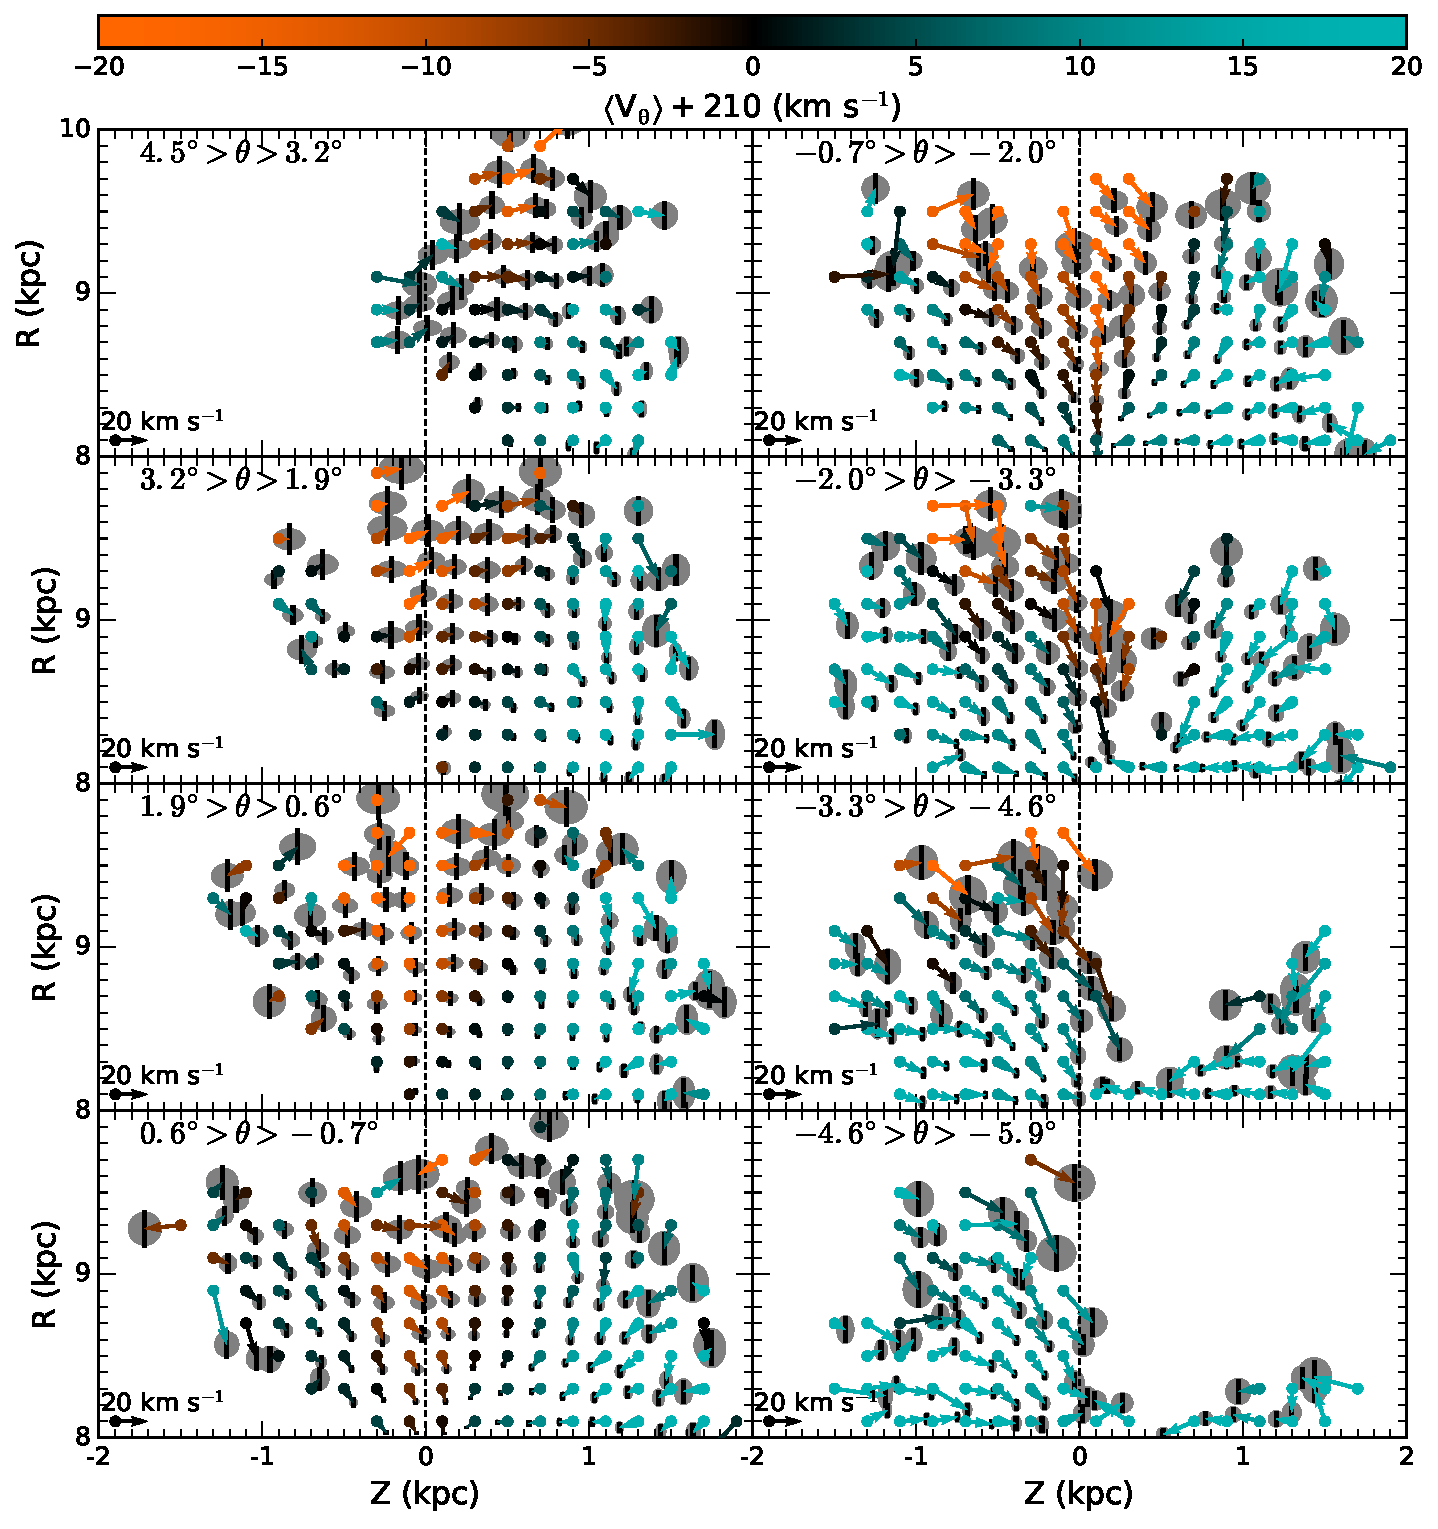
\includegraphics[width=\textwidth]{stepthetaL.pdf}
\caption{
	Comparable to Figure~11 in my paper, but contains all LAMOST stellar data, instead of only F stars. 
	\label{fig:stepthetaL}
}
\end{figure}

\begin{figure}
\centering
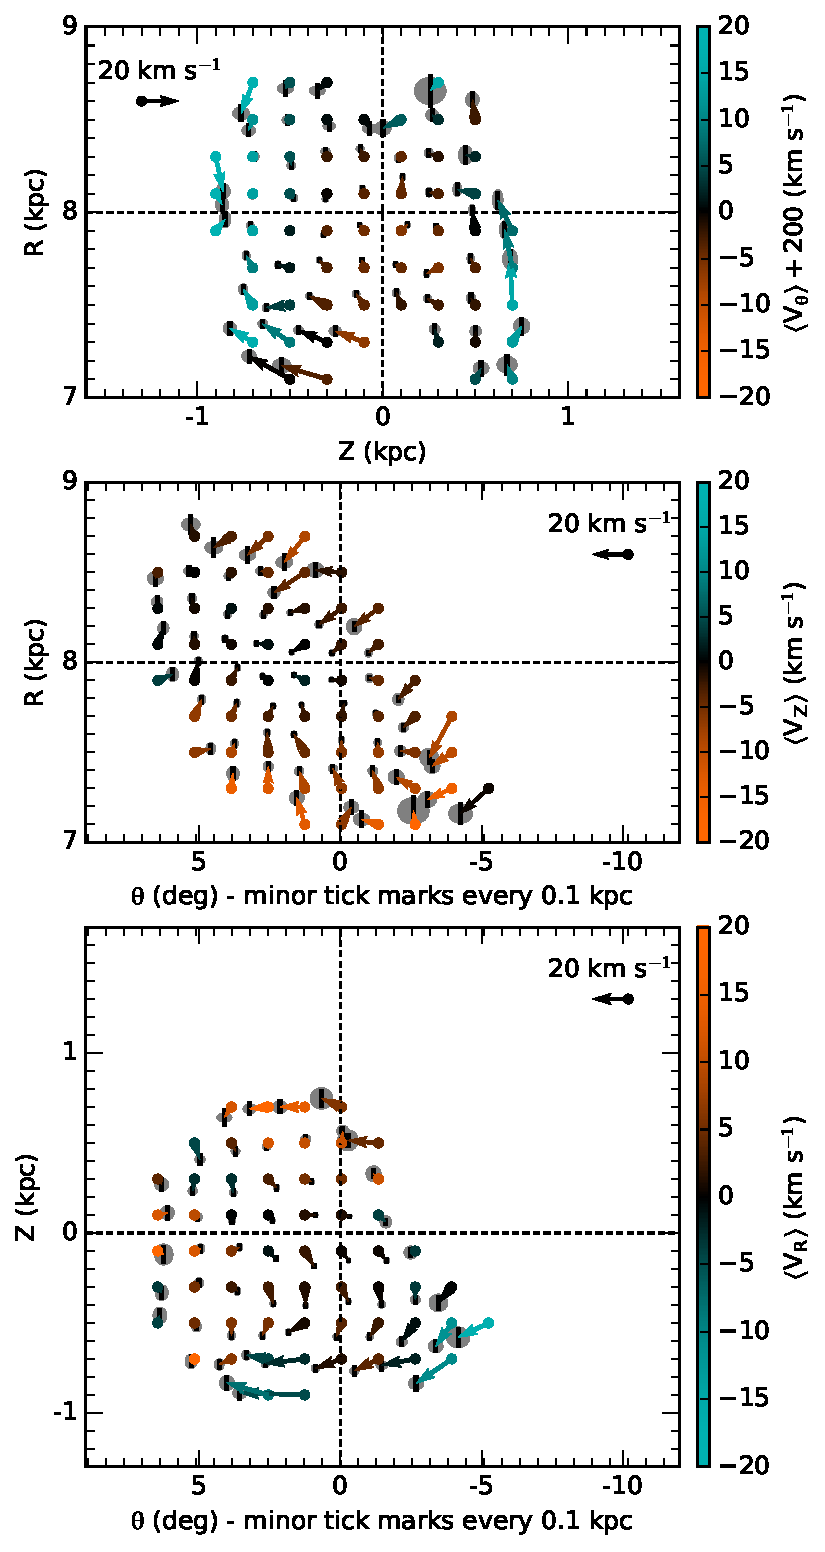
\includegraphics[width=.7\textwidth]{sideviewR.pdf}
\caption{
	Comparable to Figure~10 in my paper, but uses RAVE stellar data, instead of LAMOST. 
	\label{fig:sideviewR}
}
\end{figure}

\begin{figure}
\centering
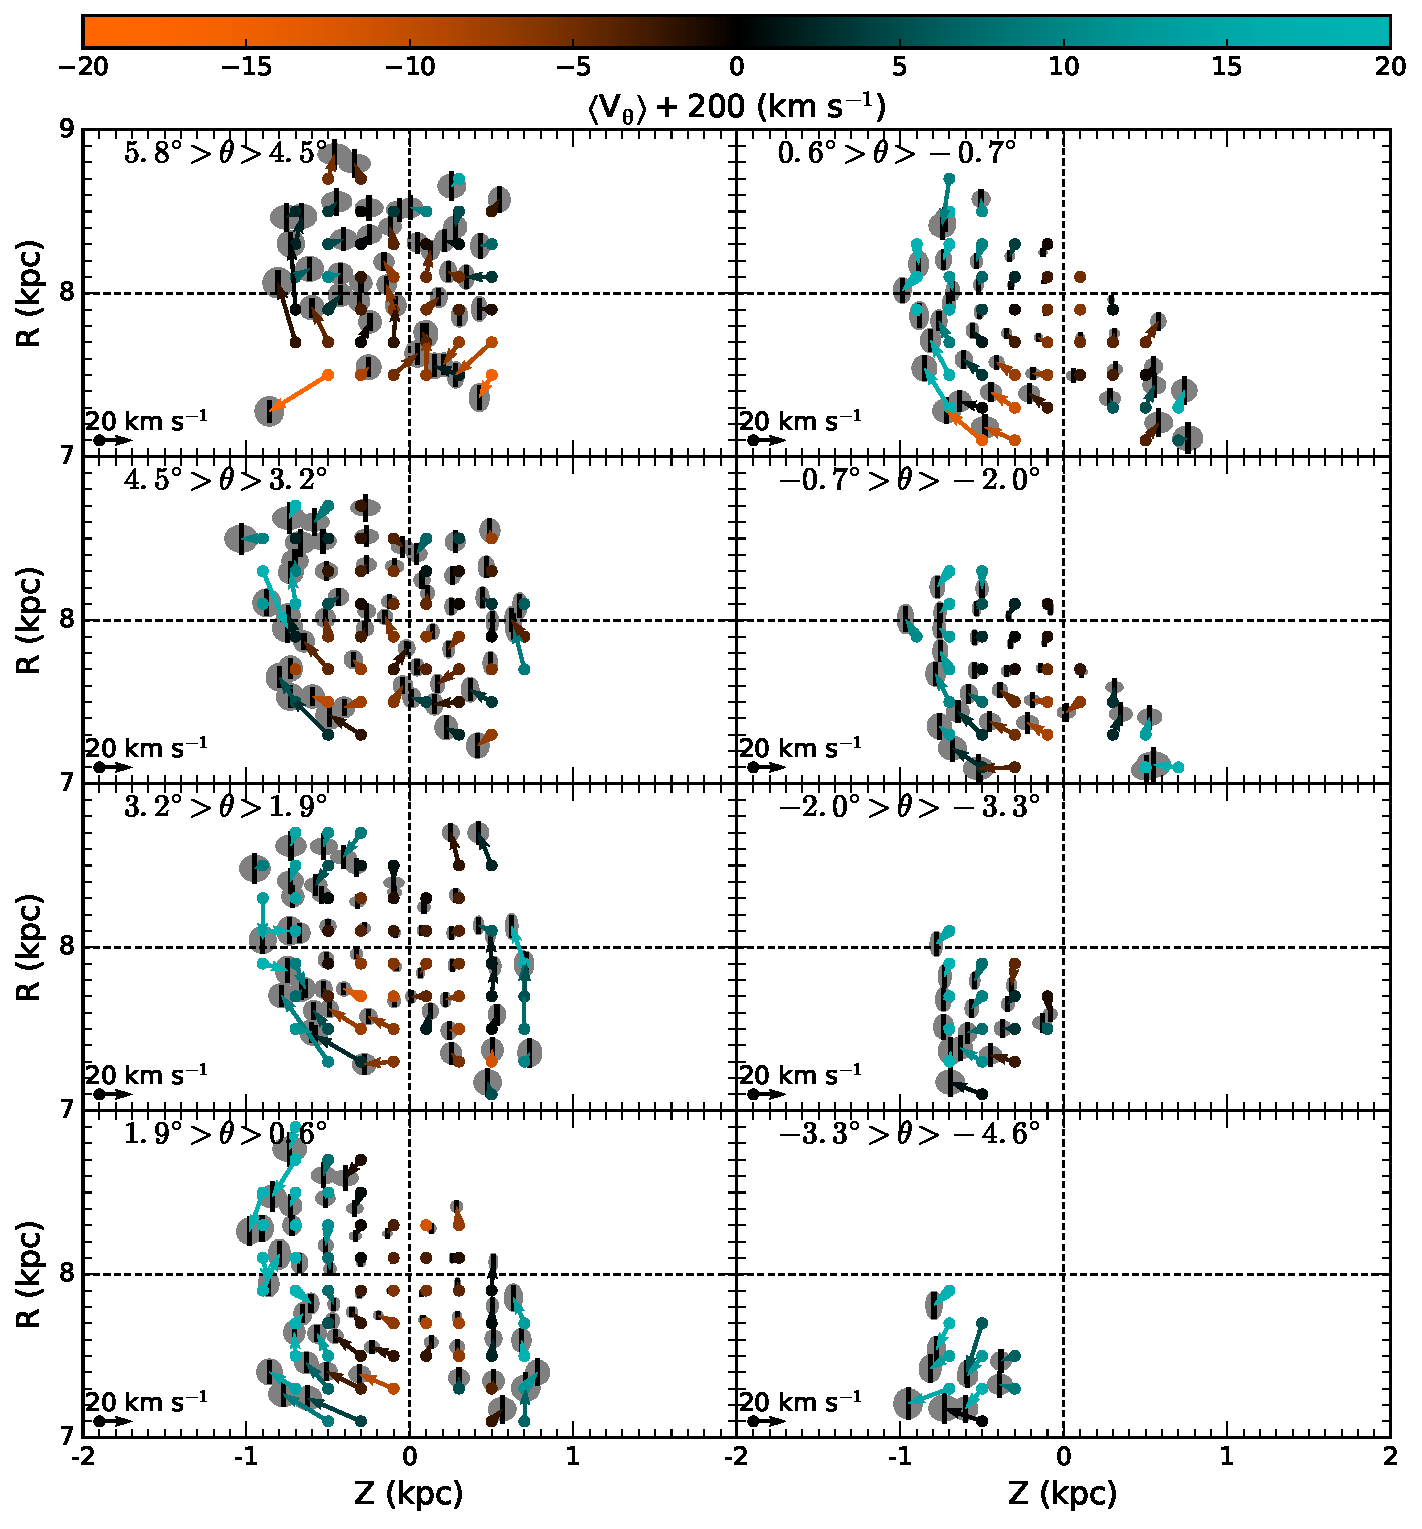
\includegraphics[width=\textwidth]{stepthetaR.pdf}
\caption{
	Comparable to Figure~11 in my paper, but uses RAVE stellar data, instead of LAMOST. 
	\label{fig:stepthetaR}
}
\end{figure}

\end{document}